\documentclass[11pt]{article}
\usepackage{memo}

% Parmaters --
\title{\large\textbf{Post-stratification weights and MR-P}}
\author{\normalsize  Shiro Kuriwaki}

\date{\normalsize October 2019}


\begin{document}
\maketitle

\onehalfspacing


The CCES 2018 Guide  reports
\begin{quote}
The [matched] cases and the frame were combined and the combined cases were balanced on multiple moment conditions using the 2017 ACS.  ... First, for the common content, the completed cases were weighted to the sampling frame using entropy balancing. ... The CCES sample was weighted to match the distributions of the 2017 ACS on gender, age, race, Hispanic origin, and education level. 

The moment conditions included age, gender, education, race, plus their interactions. The resultant weights were then post-stratified by age, gender, education, race, ``born again" status, voter registration status, and 2016 Presidential vote choice, as needed. Additionally, for the common content, the weights were post-stratified across states and statewide political races (for governor and senator). Weights larger than 15 in the common content were trimmed and the final weights normalized to equal sample size. 
\end{quote}

\begin{figure}[tbph]
\centering
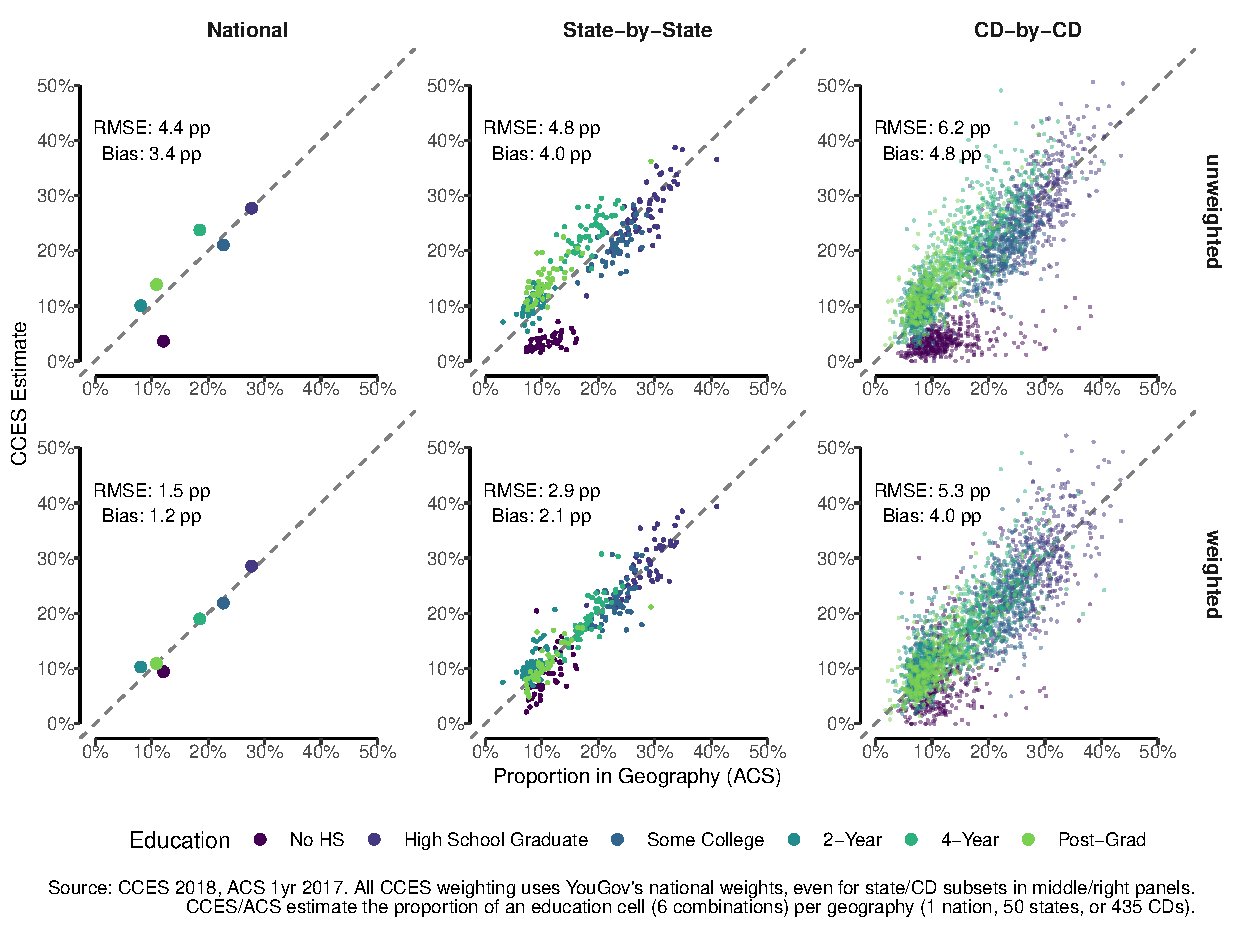
\includegraphics[width = \textwidth]{figures/educfrac-comparisons.pdf}
\end{figure}

\begin{figure}
\centering
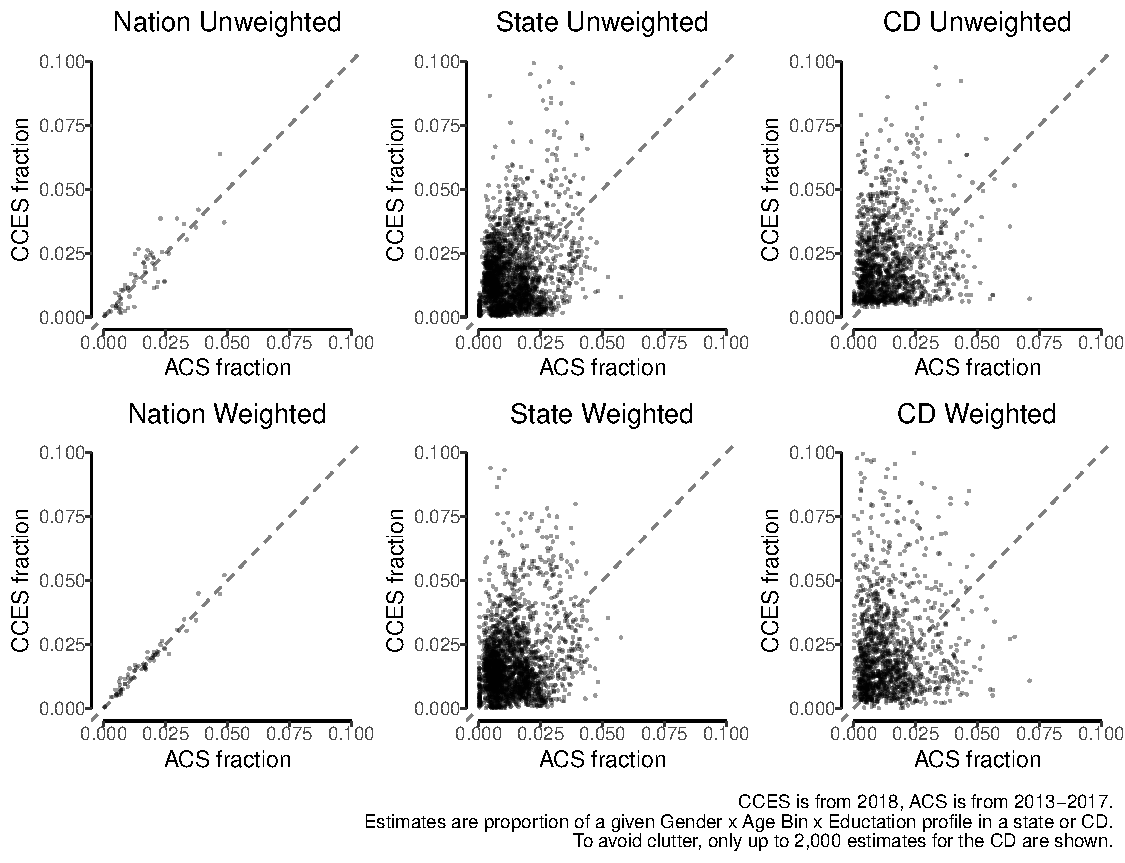
\includegraphics[width = \textwidth]{figures/cellfrac-comparisons.pdf}
\end{figure}

\end{document}



